\documentclass{article}
\usepackage{animate}
\usepackage{cancel}
\usepackage{float}
%\usepackage{gensymb}
\usepackage[margin=1in, top=1in, bottom=1in]{geometry}
\usepackage{graphicx}
\usepackage{hyperref}
\usepackage{listings}
\usepackage{tikz}
\usepackage{tikzit}
% \usetikzlibrary{external}
% \tikzexternalize[optimize=false,prefix=figures/cache/] % activate and define figures/ as cache folder
% These fix ``Too many math alphabets'' error
% See https://tex.stackexchange.com/questions/3676/too-many-math-alphabets-error
\newcommand\hmmax{0}
\newcommand\bmmax{0}

\usepackage{amsmath,amsthm,amssymb,mathabx}
\usepackage{xspace,enumerate,color,epsfig} 
\usepackage{graphicx}
%\usepackage{braket}

\usepackage{stmaryrd}
\usepackage{mathrsfs}

\usepackage{keycommand}
\usepackage{microtype}

\usepackage{url}

\usepackage[utf8]{inputenc}
\usepackage{scrextend}
\usepackage[english]{babel}

\usepackage{xcolor}
\definecolor{zx_green}{rgb}{216,248,216}
\definecolor{zx_red}{rgb}{232,165,165}

\usepackage{tikzit}
\input{zx.tikzstyles}
\input{zx.tikzdefs}

\newcommand{\R}{\mathbb{R}}
\newcommand{\C}{\mathbb{C}}
\newcommand{\N}{\mathbb{N}}
\newcommand{\Z}{\mathbb{Z}}
\newcommand{\half}{\frac{1}{2}}
\newcommand{\id}{\text{id}}
\newcommand{\st}{\text{St}}
\newcommand{\eff}{\text{Eff}}

\newcommand{\cl}[1]{\overline{#1}}
\newcommand{\opp}{\text{op}}
\newcommand{\sa}{\text{sa}}


% \newcommand{\bra}[1]{\ensuremath{\left\langle #1 \right|}}
% \newcommand{\ket}[1]{\ensuremath{\left|  #1 \right\rangle}}
% \newcommand{\braket}[2]{\ensuremath{\langle#1|#2\rangle}}
% \newcommand{\ketbra}[2]{\ensuremath{\ket{#1}\!\bra{#2}}}

\usepackage{bm}

\usepackage{mathtools}
\DeclarePairedDelimiter{\ceil}{\lceil}{\rceil}
\DeclarePairedDelimiter{\floor}{\lfloor}{\rfloor}
\DeclarePairedDelimiter{\inn}{\langle}{\rangle}
\input{zx.tikzstyles}

\def\tikzscale{1.5}

\usepackage[T1]{fontenc}
\usepackage[skins,hooks,xparse,breakable]{tcolorbox}
\usepackage{xcolor}
\usepackage{chngcntr}

\newcounter{examplecounter}
\counterwithin{examplecounter}{section}

\usetikzlibrary{calc}

\definecolor{greentitle}{RGB}{61,170,61}
\definecolor{greentitleback}{RGB}{216,233,213}
\definecolor{drakgreentitle}{RGB}{24,131,80}

\DeclareTColorBox{example}{O{}o}{
    enhanced,
    breakable,
    arc=0pt,
    boxrule=0pt,
    colback=white,
    top=3em, % you can change the top spacing
    overlay unbroken and first={
        % draw box on the left
        \node[fill=greentitleback,
            font=\color{greentitle}\sffamily\bfseries\large,
            anchor=south west,
            xshift=2mm,
            yshift=-2.2em, % you can change xshift and yshift to adjust the title placement
        ] (titlebox) at (frame.north west) 
        {Example \refstepcounter{examplecounter}\theexamplecounter
        % add cross-referencing support
        \IfValueT{#2}{\label{#2}}
        };
        
        % write title on the right
        \node[font=\color{drakgreentitle}\sffamily\large, 
        anchor=west
        ] at ($(titlebox.east)+(2mm,0mm)$) {#1};
        
        % draw the vertical line on the left
        \draw[draw=greentitleback, line width=2pt] 
            (titlebox.north west-|frame.north west)--(frame.south west);
    },
    overlay middle and last={
        \draw[draw=greentitleback, line width=2pt] 
            (frame.north west)--(frame.south west);
    }
    fonttitle=\color{greentitle}\sffamily\bfseries,
}
\newcommand{\soln}{{\\[1em] \hspace{-1em}\color{greentitle}\sffamily\large Solution: \\[0.5em]}}


\theoremstyle{definition}
\newtheorem{definition}{Definition}
\newcommand*\conj[1]{\bar{#1}}
\newcommand{\abs}[1]{{\big\vert} #1 {\big\vert}}
\newcommand{\kz}[1]{\ket{\,#1\,}}
\newcommand{\kx}[1]{\ket{#1}}
\newcommand{\bz}[1]{\bra{\,#1\,}}
\newcommand{\bx}[1]{\bra{#1}}
\newcommand{\gate}[1]{\textbf{\textsf{#1}}}
\newcommand{\mkzero}{\begin{bmatrix}1\\ 0\end{bmatrix}}
\newcommand{\mkone}{\begin{bmatrix}0\\ 1\end{bmatrix}}
\newcommand{\mkplus}{\large{\frac{1}{\sqrt{2}}}\begin{bmatrix}1\\ 1\end{bmatrix}}
\newcommand{\mkminus}{\large{\frac{1}{\sqrt{2}}}\begin{bmatrix}1\\ -1\end{bmatrix}}
\newcommand{\mab}[2]{\begin{bmatrix}#1\\ #2\end{bmatrix}}
\newcommand{\transpose}{\text{T}}

\begin{document}

\tableofcontents

\section{A bit of quantum}
\subsubsection{A \textbf{bit} of information}
Say you were asked, ``Do you like pineapple on pizza?'', and you could respond only with either ``Yes'' or ``No''.
In other words, you can only give one \textbf{bit} of information in response.
A \textbf{bit} can have one of two possible values.  For example, these two values could be yes or no, true or false, on or off,...
In computers, we call these two possible values 0 and 1.  If we have many bits, we can store many possible values.

As an analogy, whenever you flip a light switch, you expect to either turn on a lightbulb, or turn off a lightbulb.
Flipping the light switch thus flips the \textbf{bit} that represents the state of the lightbulb, between ``on'' and ``off'.
Likewise, your computer is built from billions of these switches, called \textit{transistors}, like in Figure \ref{fig:tsmc}.
\begin{figure}[H]%%%note don't have permissions to use this image
	\label{fig:tsmc}
	\includegraphics[width=\columnwidth]{images/rainbowtsmc.jpg}
	\caption{This semiconductor chip made by TSMC has been magnified exorbitantly.  Each transistor in this chip is so small, that if you lined up a thousand of them from end to end, it would be smaller than the width of a human hair.}
\end{figure}

\subsection{Diagrams}
We use diagrams to describe what happens to a system over time.  We use here the convention of reading diagrams from bottom (earliest time) to top (latest time).
\subsubsection{\textbf{Boxes} and \textbf{wires}}
In diagrams, each \textbf{wire} carries information.  They can represent physical wires, such as the electrical wire which connects your light switch to your lightbulb.  They can also represent imaginary wires, such as the sound waves when you verbally answer the question, ``Do you like pineapple on pizza?''
A \textbf{box} in our diagram represents a process: something that transforms inputs into outputs.
These inputs and outputs are our wires.  Each wire has a \textbf{type}, and each input and output of a process must be of the right type.  For instance, for the process of doing laundry, the inputs and outputs are your clothes; you wouldn't put your trash through the laundry (hopefully).
We draw boxes as trapezoids; shortly, we will see why this way of drawing them is useful.

This box represents the switch process, which flips the input bit:
\begin{equation*}{\scalebox{\tikzscale}{\tikzfig{switch_process}}}\end{equation*}
\subsubsection{\textbf{States} and \textbf{tests}}
A \textbf{state} is a process with no inputs.  In our diagrams, we draw a state as an isosceles triangle with the output wires on the base of the triangle.

A lightbulb has two possible states: on and off.  If we wire up a lightbulb to our switch, flipping the switch turns on the lightbulb:
\begin{equation}
\label{eq:switch_on}
{\scalebox{\tikzscale}{\tikzfig{switch_on}}}
\end{equation}
Likewise, we can flip the switch connected to a lit lightbulb to turn it off:
\begin{equation}
\label{eq:switch_off}
{\scalebox{\tikzscale}{\tikzfig{switch_off}}}
\end{equation}
A \textbf{test}\footnote{In the wild\cite{PQP}, another word for it is \textbf{effect}.} is a process with no outputs.  When a test is applied to a state, it tests how likely the corresponding outcome is to occur.

In our diagrams, we draw a test as an upside-down state: an isosceles triangle with the input wires on the base of the triangle.  To apply a test to a state, we connect the state and the test with a wire.  This way, the output of the state is the same as the input to the test.  In total, our diagram with a test applied to a state has zero inputs and zero outputs --- this is called a \textbf{number}.  This number encodes the probability that given that state, the outcome observed is the outcome being tested for.

For our lightbulb example, when the test matches the state, this number equals 1:
\begin{equation}
{\scalebox{\tikzscale}{\tikzfig{lightbulb_test00}}}
\end{equation}

\begin{equation}
\label{eq:lightbulb_test11}
{\scalebox{\tikzscale}{\tikzfig{lightbulb_test11}}}
\end{equation}
On the other hand, when the test is the opposite of the state, this number equals 0:
\begin{equation}
{\scalebox{\tikzscale}{\tikzfig{lightbulb_test01}}}
\end{equation}
\begin{equation}
{\scalebox{\tikzscale}{\tikzfig{lightbulb_test10}}}
\end{equation}

\subsection{A \textbf{qubit} of information}
\subsubsection{Classical states and tests}
Having learned about states and tests in general, we are now ready to start tackling quantum states and tests.  Alongside gaining intuition from our diagrams, we will learn how to use \textit{bra-ket notation} (also called Dirac notation, as it was created by Paul Dirac so a physicist could represent vectors).  Thankfully, this new jargon is simple: kets are what we call states, and bras are what we call tests.

Just as a bit is the smallest unit of information in a computer, a \textbf{qubit} is the smallest unit of information in a quantum computer.
We can encode any bit as a qubit by mapping a bit with value 0 to the $\kz0$ (pronounced ``ket 0'') qubit state, and a bit with value 1 to the $\kz1$ (pronounced ``ket 1'') qubit state.  These are defined as:
\begin{align}
\label{eq:ket0}
&\tikzfig{ket0}\\
\label{eq:ket1}
&\tikzfig{ket1}
\end{align}

Let us plot them on the unit circle of the real 2D plane.
\begin{figure}[H]
	\ctikzfig{unitcircle01}
	\caption{$\kz0$ and $\kz1$ are plotted here on the unit circle.  This is just directly plotting their statevectors in 2D.}
	\label{fig:unitcircle}
\end{figure}
Let us note a few of their properties:
\begin{itemize}
\item They are \textit{orthogonal}: on the unit circle there is a right angle between them.
\item They are \textit{normalized}: they have a vector norm, or length, of 1.
\item They \textit{span} the real 2D plane: you can get any arbitrary 2D vector $\vec{v}$ of real numbers by taking their linear combination
\begin{align}
	\ket{v} &= a \kz0 + b \kz1\\
	&= a \mkzero + b \mkone\\
	&= \mab{a}{b}
\end{align}
where $a$ and $b$ are complex numbers\footnote{Mathematicians might call them coefficients, and physicists might call them probability amplitudes.}.
\end{itemize}
They form an \textbf{orthonormal basis} for $\mathbb{R}_2$, the \textit{vector space} of real 2D vectors.
We call this basis the \textbf{computational basis} because they encode a qubit as a bit.

Apart from the unit circle, another way to visualize these two states is on a sphere called the \textbf{Bloch sphere}, which looks like:
\begin{figure}
	\ctikzfig{blochxyz}	
	\caption{This is what the Bloch sphere looks like.}
	\label{fig:blochsphere}
\end{figure}
In addition to calling this basis for qubit states the computational basis, we also call it the \textbf{Z basis}.  This is because the states $\kz0$ and $\kz1$, called the \textit{Z-basis states}, are respectively on the positive and negative z-axis of the Bloch sphere.
\begin{figure}
	\ctikzfig{bloch01}
	\caption{$\kz0$ and $\kz1$ are plotted here on the Bloch sphere.}
\end{figure}
You might notice that on the Bloch sphere, the angle between these two states is $\pi$, or $180^{\degree}$.  However, when you take the inner product of the vectors in Equations \ref{eq:ket0} and \ref{eq:ket0}, or plot them on the unit circle as in Figure \ref{fig:unitcircle}, the angle between these two states' vectors is $\frac{\pi}{2}$ radians ($90^{\degree}$).
Indeed, any angle on the Bloch sphere is twice what it would be if we had plotted the vector in 2D.
While this may seem like an unnecessary complication now, we will later see how the Bloch sphere helps us visualize when our qubit states contain \textit{complex numbers}.
Throughout this text we will use radians instead of degrees, and adopt the convention of angles being angles on the Bloch sphere.

\subsubsection{The qubit NOT gate}
Recall how earlier in Equations \ref{eq:switch_on} and \ref{eq:switch_off}, we modelled how a light switch is a process which turns on an off lightbulb, and turns off an on lightbulb?
That is the NOT operation on a bit.
On a qubit, we also have a NOT operation which behaves as you expect:
\begin{equation}
	\tikzfig{ket0switch}
\end{equation}
\begin{equation}
	\tikzfig{ket1switch}
\end{equation}
When your qubit is in one of the classical states (corresponding to the two possible values a bit can have on a classical computer), the NOT gate is the bit flip gate: if you interpret 0 as false and 1 as true, then not true is false and not false is true.  The NOT gate flips the $\kz0$ state to the $\kz1$ state, and the $\kz1$ state to the $\kz0$ state.

What does the NOT gate do to a qubit state in general?  What it does is rotate the state vector on the Bloch sphere half a rotation about the x-axis; the axes are labelled in Figure \ref{fig:blochsphere}.  That is why the NOT gate is also called the \textbf{X gate}, as we will call it from now on.

As in our lightbulb example, when we flip a diagram of a state upside-down, we get a diagram of a test.
Flipping our diagrams of $\kz0$ and $\kz1$ in Equations \ref{eq:ket0} and \ref{eq:ket1} upside-down gives $\bz0$ (``bra 0'') and $\bz1$ (``bra 1'') respectively:
\begin{align}
&\tikzfig{bra0}\\
&\tikzfig{bra1}
\end{align}

We can connect the wire from state to test to get a number:
\begin{align}
	&\tikzfig{braket00} \label{eq:braket00} \\
	&\tikzfig{braket01} \label{eq:braket01} \\
	&\tikzfig{braket10} \label{eq:braket10} \\
	&\tikzfig{braket11} \label{eq:braket11} 
\end{align}
This number is the \text{inner product} of the bra vector and the ket vector.

You can observe one similarity between bra-ket notation here and conditional probability: the notation of a vertical line in-between.  For events \textsf{A} and \textsf{B},
\begin{equation}
	\text{Pr}(\,\textsf{A}\,|\,\textsf{B}\,) \coloneqq \text{Probability of \textsf{A} given \textsf{B}}
\end{equation}
This is by design.  In general, given a \textit{normalized}\footnote{We'll give a mathematical definition of this later.  Intuitively, you want your states and tests to be normalized so that you don't break the rules of the universe governing probabilities.} state $\ket{\,s\,}$ and test $\bra{\,t\,}$ pair, the probability that you observe the outcome $\bra{\,t\,}$ you were testing for, given the state is $\ket{\,s\,}$, is
\begin{equation}
	\label{eq:braketprob}
	\text{Pr}(\,t\,|\,s\,) = \abs{\langle \,t\,|\,s\,\rangle}^2
\end{equation}
This inner product is also called a \textbf{probability amplitude}, or amplitude for short.  The word "probability" follows form how you can always calculate the probability given a probability amplitude using Equation~\ref{eq:braketprob}, i.e. the probability is the \textit{norm-squared} of the probability amplitude.  This definition applies even when the probability amplitudes are complex numbers.  For now, we will stick with probability amplitudes which are real numbers, in which case the probability is simply the probability amplitude squared.

On the other hand, it can help to think of the word "amplitude" visually.  When you have a state drawn on the unit circle, you can draw a vertical line to the x-axis.  The height of the right triangle you just formed is the probability amplitude when you test for the $\kz1$ state given your state.  Likewise, the base of that right triangle is the probability amplitude when you test for the $\kz0$ state.
\begin{figure}[H]
	\ctikzfig{unitcircletrinoangle}
	\caption{A one qubit statevector $\kx{v}$ plotted on the unit circle.  The vector $\vec{v}$ forms the hypotenuse of a right triangle with sides of length $\abs{a}$ and $\abs{b}$.  Testing for the Z-basis states results in probability amplitudes of $\langle \,0\,|\,v\,\rangle = a$ and $\langle \,1\,|\,v\,\rangle = b$.}
	\label{fig:unitcircletrinoangle}
\end{figure}

\subsubsection{The X-basis states}
We have gotten comfortable with the qubit states which encode the classical bit states 0 and 1.  Yet if all we do with qubits is represent binary values, we are using a quantum bit to do exactly what a classical bit does.  We now demystify the math of one of the key features of quantum computing: \textit{superposition}.
A qubit is more powerful than a bit.  Informally, it can be 0, 1, or ``anything in-between''.  \textbf{Superposition} is this property of quantum states to encode information ``in-between'' states.  You might also hear people call a superposition of states, a \textit{mixture} of states.

A thought experiment about quantum superposition that you may have heard of before is Schr\"odinger's cat.  Suppose you have a closed box, and you know there is a cat in that box.  The question is, is that cat alive or dead?  The only way for you to tell is to open the box:
\noindent%
\begin{minipage}[t]{0.45\linewidth}
	\begin{frame}{}
		\animategraphics[controls,width=2in]{12}{images/OpeningBox/animation-}{0}{271}
	\end{frame}
\end{minipage}
More formally, you know that the cat in the box is in one of two states: alive or dead.
At the moment before you look into the box, your knowledge of the state of the cat is in superposition: there is some probability that the cat turns out to be alive, and some probability that the cat turns out to be dead.
The act of seeing the cat allows you to confirm which state of these two states the cat is in.

We will start with a special case of superposition that we will see often: that of \textit{equal superposition}.  Consider the state
\begin{equation}
	\tikzfig{ket+unnorm}
	\label{eq:ket+unnorm}
\end{equation}

It is the sum of $\kz0$ and $\kz1$:
\begin{equation}
	\tikzfig{ket+unnormsuperposition}
	\label{eq:ket+unnormsuperposition}
 \end{equation}

However, we will notice something goes wrong when we try to test the $\ket{+}$ state for itself:
\begin{equation}
	\tikzfig{braket++unnorm}
	\label{eq:braket++unnorm}
\end{equation}
We should have gotten the number 1, corresponding to probability 1, but instead we got a number greater than 1.
Somehow, we have calculated a probability of more than 1!
To fix this error, we need to introduce the concept of \textit{normalization}.
That means that we need to multiple our states by a constant factor so that if you test the state for itself, your test is successful 100\% of the time.
The $\kz0$ state is already normalized, as we saw in Equation~\ref{eq:braket00}.
To ensure the $\ket{+}$ state is normalized, we multiple by a factor of $\frac{1}{\sqrt{2}}$, which we will soon see fixes that issue.

The $\ket{+}$ state is one of the \textbf{X-basis} states.  Just as the Z-basis states lie on the Z axis of the Bloch sphere, the X-basis states lie on the X axis of the Bloch sphere.
We also introduce the other X-basis state, the $\ket{-}$ state.
\begin{align}
\label{eq:ket+}
&\tikzfig{ket+}\\
&\tikzfig{ket-}
\label{eq:ket-}
\end{align}

Like the $\kz0$ and $\kz1$ states, the $\kx+$ and $\kx-$ states can also be plotted on the unit circle:
\begin{figure}[H]
	\ctikzfig{unitcircle+-}
	\caption{$\kx+$ and $\kx-$ are plotted here on the unit circle.  This is just directly plotting their statevectors in 2D.}
	\label{fig:unitcirclexbasis}
\end{figure}

Perhaps you can guess what happens when given an X-basis state, you test for an X-basis state. Hint: it's the same as what happened with the Z-basis states in Equations~\ref{eq:braket00}~to~\ref{eq:braket11}.\nopagebreak
\begin{align}
	&\tikzfig{braket++}\\
	&\tikzfig{braket--}\\
	&\tikzfig{braket+-}\\
	&\tikzfig{braket-+}
\end{align}

On the Bloch sphere, they are on the positive and negative x-axis:
\begin{figure}[H]
	\ctikzfig{bloch+-}
	\caption{$\kx+$ and $\kx-$ are plotted here on the Bloch sphere.}
\end{figure}

You can think of the X-basis states as being exactly ``halfway in-between'' the Z-basis states.  Indeed, on the Bloch sphere, $\kz0$ and $\kz1$ are respectively on the north and south poles, while $\kx+$ and $\kx-$ are on the equator:
\begin{figure}[H]
	\ctikzfig{bloch+-wrt01}
	\caption{All states ``halfway in-between'' $\kz0$ and $\kz1$, such as $\kx+$ and $\kx-$, lie on the equator of the Bloch sphere.}
\end{figure}

In other words, the X-basis states are both \textbf{superpositions}, i.e. a complex linear combination, of the Z-basis states:
\begin{align}
\ket{+} &= \frac{1}{\sqrt{2}} (\kz0 + \kz1) \label{eq:kp01} \\
\ket{-} &= \frac{1}{\sqrt{2}} (\kz0 - \kz1) \label{eq:km01} \\
\end{align}
Nicely, the Z-basis states are in turn both superpositions of the X-basis states:
\begin{align}
\kz0 &= \frac{1}{\sqrt{2}} (\ket{+} + \ket{-}) \label{eq:k0pm} \\
\kz1 &= \frac{1}{\sqrt{2}} (\ket{+} - \ket{-}) \label{eq:k1pm}
\end{align}

Furthermore, Equations~\ref{eq:kp01}~to~\ref{eq:k1pm} above are \textit{uniform} superpositions --- each probability amplitude (i.e. coefficient) has the same magnitude of $\frac{1}{\sqrt{2}}$.
What this means is that the inner product of an X-basis state with a Z-basis state has magnitude $\frac{1}{\sqrt{2}}$:
\begin{align}
&\tikzfig{braket0+} \label{eq:braket0+} \\
&\tikzfig{braket1+}\\
&\tikzfig{braket0-}\\
&\tikzfig{braket1-} \label{eq:braket1-}
\end{align}
As we learned in Equation \ref{eq:braketprob}, the norm-squared of the probability amplitude is the probability you observe the outcome you're testing for.    Let's see this through an example.

\begin{example}[]
\label{ex:pr1m}
If your state is $\kx-$, and you test for $\kz1$, what is the probability you observe $\kz1$?

\textnormal{From Equation \ref{eq:braketprob}, we know that the probability of observing $\kz1$ when the state is $\kx-$ is $\abs{\langle\,1,\,|-\rangle}^2$.  In Equation \ref{eq:braket1-}, we found that $\langle\,1,\,|-\rangle = \texttt{-}\frac{1}{\sqrt{2}}$.  Therefore, the probability is $\abs{\langle\,1,\,|-\rangle}^2 = \frac{1}{2}$.}
\end{example}

You'll find that if you test for $\kz0$ when the state is $\kx-$, the probability is also $\frac{1}{2}$.  We've now arrived at the physical meaning of why we say that the X-basis states are ``halfway in-between'' the Z-basis states!  This leads us to the very important of quantum measurement...

\subsection{Quantum Measurement}
So far, we have talked about the mathematical description of the Z- and X- basis qubit states.  Now, let's talk about what is going on physically.
All around us are ``quantum states''.  You are made up of perhaps an octillion ($10^{27}$) molecules.  At any time, each molecule has its own quantum state.  However, in our macroscopic (at least compared to the length scale of individual molecules) world, we simply observe the collection of those molecules --- you!

Quantum effects only become relevant at really tiny length scales.  The size of today's transistors is just about small enough that quantum effects come into play.
\textit{Classical mechanics} is sufficient to describe most of physics on the length scale of us humans.  We need \textit{quantum mechanics} to describe physics on the length scale of atoms and molecules.

\subsubsection{The First Quantum Measurement Experiment}
To explore quantum measurement, we'll start with one of the earliest experiments in the history of quantum physics: the Stern-Gerlach experiment~\cite{Gerlach_Stern_1922}.  In fact, it was the first experiment where separate quantum states were directly observed!

Otto Stern designed this experiment, which Walther Gerlach carried out, where silver atoms were sent through an inhomogenous (different strength at different points in space) magnetic field and then hit a detector screen.  What happened, was that half of the atoms were deflected up, and half of the atoms were deflected down.  Interestingly, none of the atoms were observed at the height in-between.  This suggested that each silver atom had as an intrinsic property specifying which of the two directions it would be deflected in this experiment.  This property is \textbf{quantized} because when it is observed, its possible values are discrete rather than a continuous distribution.  If the atoms were instead spinning magnetic dipoles, they would be deflected by the magnetic field in a direction according to their spin, although the physics are different.  Due to this analogy, this quantized value of the atom is called \textit{spin}.

Due to the magnetic field (say it's oriented so its north pole is in the $+$z direction), atoms in a spin up quantum state would be deflected one way (up), and atoms in a spin down quantum state would be deflected the opposite way (down).

Up to now, given a qubit state, we have computed the probabilities of observing a certain outcome that we are testing for.  We will now learn about \textbf{orthonormal basis (ONB) measurement} --- a type of \textbf{quantum measurement} in which you observe exactly one of the outcomes in your chosen orthonormal basis of quantum states.  This is the type of quantum measurement you will use the most as a quantum computer scientist.  This is also the type of measurement done by the inhomogenous magnetic field in the Stern and Gerlach experiment.

When you perform an ONB measurement, you are actually simultaneously testing for all of the states in your ONB.  You can only observe one of those states, which is your measurement outcome.  The probability of you observing each outcome is exactly as how we have been computing so far: taking the norm-squared of the braket between your test (one of the states in your orthonormal basis) and your quantum state.

After your ONB measurement, \textit{your state becomes the one that was your measurement outcome}.  Doesn't matter if your state was not one of the ones in your ONB --- if that case, the act of performing quantum measurement changes the very state you are measuring.

At first, this may seem counterintuitive to our macroscopic world.  If you hold a ruler to find the position of a pin, you wouldn't expect the ruler to change where the pin is.  However, just to see the pin, you need to shine light on it.  Light is made up of photons which have momentum.  This momentum does nothing, as far as our eye can tell, to a massive (compared to the photon) object like the pin, but if it was instead a much smaller object with size comparable to that of photons, the momentum could be absorbed by it.  Therefore, your act of trying to see the pin can change the state of the pin.
%%% need to refine this explanation, create a ``collapse'' image, and create a unit circle trig image

As we saw from Example \ref{ex:pr1m}, the Z- and X- bases have the property that when measured in the other of the two bases, the probability of any measurement outcome is uniformly $\frac{1}{2}$.  For this reason, the Z- and X- bases are called \textit{mutually unbiased bases} with respect to each other.  We've now learned enough about mathematically describing quantum two-state systems to combine that understanding with what Stern and Gerlach observed.

\begin{example}[Z-measurement then Z-measurement] \label{example:sterngerlachzz}
Stern and Gerlach observed that each silver atom passing through their inhomogenous magnetic field in the z direction had a $\frac{1}{2}$ chance of being deflected upwards ($+$z direction), and a $\frac{1}{2}$ chance of being deflected downwards ($-$z direction).  They then took each silver atom that was deflected upwards, and sent that through another inhomogenous magnetic field in the z direction.  This second time, all the atoms were deflected upwards --- why?

\begin{figure}[H]
	\ctikzfig{sterngerlachzz}
	\caption{This is what Stern and Gerlach saw when they sent a beam of silver atoms through the experimental setup of Example \ref{example:sterngerlachzz}.}
\end{figure}

\textnormal{All of the atoms deflected upwards by the first field (which was in the z-direction) were in the $z_+$ (spin up with respect to the z-axis) state, which we'll represent as the $\kz0$ state because the $\kz0$ state points in the $+$z direction on the Bloch sphere.  After those $z_+$ atoms traversed the second field (which was also in the z-direction), the probability of observing $z_+$ was
\begin{equation}
	\label{eq:prob00}
	\text{Pr}(\,0\,|\,0\,) = \abs{\langle\,0\,|\,0\,\rangle}^2
\end{equation}
From Equation \ref{eq:braket00}, we know that $\langle\,0\,|\,0\,\rangle$ is 1.  Therefore, all atoms that were deflected upwards after the first field, were also deflected upwards after the second field.}

\textnormal{Following this logic, we expect that any number of Z-measurements done thereafter would continue to yield the $z_+$ state.}
\end{example}

\begin{example}[Z-measurement then X-measurement] \label{example:sterngerlachzx}
	Stern and Gerlach observed that each silver atom passing through their inhomogenous magnetic field in the z direction had a $\frac{1}{2}$ chance of being deflected upwards ($+$z direction), and a $\frac{1}{2}$ chance of being deflected downwards ($-$z direction).  They then took each silver atom that was deflected upwards, and sent that through another inhomogenous magnetic field, this time in the x direction.  This second time, $\frac{1}{2}$ the atoms were deflected in the $+$x direction and $\frac{1}{2}$ the atoms were deflected in the $-$x direction --- why?
	
	\begin{figure}[H]
		\ctikzfig{sterngerlachzx}
		\caption{This is what Stern and Gerlach saw when they sent a beam of silver atoms through the experimental setup of Example \ref{example:sterngerlachzx}.}
	\end{figure}

	\textnormal{Again, we use the $\kz0$ state to represent $z_+$, all atoms deflected upwards by the first field.  The $\kx+$ and $\kx-$ states are suitable to represent $x_+$ and $x_-$, the state of all atoms after the x-aligned magnetic field, because these states point in the $+x$ and $-x$ directions on the Bloch sphere.	After those $z_+$ atoms traversed the second field (in the x-direction), the probability of observing $x_+$ was
	\begin{equation}
		\text{Pr}(x_+|z_+) = \text{Pr}(+|\,0\,) = \abs{\langle+|\,0\,\rangle}^2
	\end{equation}
	and the probability of observing $x_-$ was
	\begin{equation}
		\text{Pr}(x_-|z_+) = \text{Pr}(-|\,0\,) = \abs{\langle-|\,0\,\rangle}^2
	\end{equation}
	From Equation \ref{eq:braket0+}, we know that $\langle+|\,0\,\rangle = \conj{\langle\,0\,|+\rangle} = \conj{\frac{1}{\sqrt{2}}} = \frac{1}{\sqrt{2}}$.  Likewise, $\langle-|\,0\,\rangle = \frac{1}{\sqrt{2}}$.  Therefore, all atoms that were deflected upwards after the first field, had a 50-50 chance of being deflected left or right after the second field.}
\end{example}

\begin{example}[Z-measurement then X-measurement then Z-measurement] \label{example:sterngerlachzxz}
	After their setup in Example \ref{example:sterngerlachzx}, Stern and Gerlach sent the $x_+$ silver atoms through one more z-aligned inhomogenous magnetic field.  They were surprised at what they saw.  What did they see?
	
	\begin{figure}[H]
		\ctikzfig{sterngerlachzxz}
		\caption{This is what Stern and Gerlach saw when they sent a beam of silver atoms through the experimental setup of Example \ref{example:sterngerlachzxz}.}
	\end{figure}

	\textnormal{At the end of Example \ref{example:sterngerlachzx}, the state was $x_+$, which we worked out is the $\kx+$ state.  After those $x_+$ atoms traversed the third field (in the z-direction), the probability of observing $z_+$ was
	\begin{equation}
		\text{Pr}(z_+|x_+) = \text{Pr}(\,0\,|+) = \abs{\langle\,0\,|+\rangle}^2
	\end{equation}
	and the probability of observing $z_-$ was
	\begin{equation}
		\text{Pr}(z_-|x_+) = \text{Pr}(\,1\,|+) = \abs{\langle\,1\,|+\rangle}^2
	\end{equation}
	From Equation \ref{eq:braket0+}, we know that $\langle\,0\,|+\rangle = \frac{1}{\sqrt{2}}$.  Likewise, $\langle\,1\,|+\rangle = \frac{1}{\sqrt{2}}$.  Therefore, all atoms that were in the $\kx+$ state after the second field, had a 50-50 chance of being deflected up or down by the third field.  Therefore, the reason for Stern and Gerlach's surprise was that although the second of two consecutive Z-measurements yielded all $\kz0$ as we saw in Example \ref{example:sterngerlachzz}, adding an X-measurement in-between the Z-measurements changed that to half $\kz0$ and half $\kz1$.}
\end{example}

\newpage
\subsection{The pure qubit state, in general}
So far we have seen several examples of one-qubit states depicted on the unit circle and the Bloch sphere.  What do you need to depict any one-qubit state in general?

\subsubsection{Statevectors on the unit circle}
Any vector $\kx{v}$ on the unit circle by definition has magnitude (length) 1.
Its general form is
\begin{equation}
	\label{eq:onequbitpurerealform}
	\tikzfig{ketv}
\end{equation}
where $a$ and $b$ are real numbers.
When you perform a Z-basis measurement on a qubit whose statevector is of this form, according to Equation \ref{eq:braketprob}, the probability your outcome is $\kz0$ is
\begin{align}
	\text{Pr}(\,0\,|\,v\,) &= \abs{\langle \,0\,|\,v\,\rangle}^2\\
	&= \abs{\bz0 \text{\large(}a\kz0 + b\kz1\text{\large)}}^2\\
	&= \abs{a\,\langle \,0\,|\,0\,\rangle + b\,\langle \,0\,|\,1\,\rangle}^2\\
	&= \abs{a + 0}^2\\
	&= a^2
\end{align}
Likewise, the probability your outcome is $\kz1$ is $b^2$.  Since the only possible outcomes are $\kz0$ and $\kz1$, probability is conserved:
\begin{equation}
	a^2 + b^2 = 1
\end{equation}
Let's review how we draw this geometrically, as we did in Figure~\ref{fig:unitcircletrinoangle} back when we first introduced probability amplitudes.  It helps to draw a right triangle where the hypotenuse is $\kx{v}$, and the sides are parallel with $\kz0$ and $\kz1$.
Hence when $a$ and $b$ are real numbers, it is convenient to remember that the probabilities working out is simply the Pythagorean theorem:
\begin{equation}
	a^2 + b^2 = c^2
	\label{eq:pythagorean}
\end{equation}
where $a$ and $b$ are sides of the right triangle and $c$ is the hypotenuse.  In our case of a normalized vector on the unit circle, it has to have length 1, i.e. $c = 1$.
\begin{figure}[H]
	\ctikzfig{unitcircletriangle}
	\caption{A one qubit statevector $\kx{v}$ of the form $a\kz0 + b\kz1$, where $a$ and $b$ are real numbers, plotted on the unit circle.  The vector $\vec{v}$ forms the hypotenuse of a right triangle with sides of length $\abs{a}$ and $\abs{b}$.  The $a$ and $b$ shown in this figure are positive, but they can be any numbers from $-1$ to $1$ inclusive as long as they satisfy Equation~\ref{eq:pythagorean}, meaning they are on the unit circle.}
	\label{fig:unitcircletriangle}
\end{figure}


\subsubsection{Statevectors on the Bloch sphere}
The unit circle is not sufficient for our purposes.  That is because in general, a pure one qubit statevector is of the form
\begin{equation}
	\label{eq:onequbitpuregenform}
	\tikzfig{ketpsi}
\end{equation}
where $\alpha$ and $\beta$ are complex numbers.
Hence compared to Equation \ref{eq:onequbitpurerealform}, what's new is that coefficients can have imaginary components.  We celebrate this by chopping off the left corner of the triangle in our diagrams.  This will allow us to pictorially represent some key properties of complex vectors, as we will explore in the next section.

We mentioned earlier that going from the unit circle to the Bloch sphere, you double the angles.  We can see this by looking at the slice of the Bloch sphere where the unit circle lives, outlined as a black circle in Figure~\ref{fig:unitcircleinbloch}.
Plotting the same statevector, the angle $\theta$ on the Bloch sphere in Figure~\ref{fig:unitcircletriangle} is twice the angle $\Theta$ on the unit circle in Figure \ref{fig:unitcircleinbloch}, i.e. $\theta = 2 \Theta$.

We can always plot a statevector with real coefficients on the Bloch sphere in three steps:
\begin{enumerate}
	\item Find the angle $\Theta = \text{arctan}(\frac{b}{a})$
	\item Double that angle to get $\theta = 2 \Theta$
	\item Starting from the $+z$ axis (where $\kz0$ is), rotate an angle of $\theta$ along this slice of the Bloch sphere where the unit circle lives
\end{enumerate}

\begin{figure}[H]
	\ctikzfig{unitcircleinbloch}
	\caption{\textbf{Left:} A pure one qubit statevector $\kx{\psi}$ has the general form $\alpha\kz0 + \beta\kz1$, where $\alpha$ and $\beta$ are complex numbers.  Here, $\kx{\psi}$ is plotted on the Bloch sphere for the case where both $\alpha$ and $\beta$ are real numbers, and thus $\kx{\psi}$ must be in the XZ plane of the Bloch sphere, and lie on the circle outlined here in black.  \textbf{Right:} The unit circle plotted on the 2D real plane, as plotted in Figure~\ref{fig:unitcircletriangle}.}
	\label{fig:unitcircleinbloch}
\end{figure}
So if vectors on the Bloch sphere whose coefficients are real numbers lie on that circle, what about the rest of the sphere?
The rest of the sphere is where the coefficients have imaginary components.
Before we talk about the general form of any vector on the Bloch sphere, let us first get comfortable with probability amplitudes being complex numbers.

Up until now, to obtain the test corresponding to a state, all we had to do was take the matrix transpose of the ket column vector to get the bra row vector.  That has been correct so far because we have been dealing just with real numbers.  In general, when the statevectors can have complex coefficients, we need to take the \textit{conjugate transpose}\footnote{As a refresher, this means to take the transpose where you also replace each number by its complex conjugate.  This way, when all the numbers are real, the conjugate transpose and transpose operations are identical.} of the ket to get the bra, and the conjugate transpose of the bra to get the ket.

In the following example, we will introduce how we can perform transformations on our diagrams which correspond to transformations on our matrices.
\begin{example}[Y-basis states]
	What are the statevectors and diagrams corresponding to the complex conjugation, transpose, and conjugate transpose of $\kx{+i}$ and $\kx{-i}$, the Y-basis states introduced below?

	\textnormal{While we have seen the Z- and X- basis states in action, we have yet to do anything with the y axis of the Bloch sphere.
	The $+$y and $-$y axes respectively define two Y-basis states:
	\begin{align}
		\label{fig:ket+i}
		\tikzfig{ket+i}\\
		\label{fig:ket-i}
		\tikzfig{ket-i}
	\end{align}
	It doesn't make sense to visualize this on the unit circle, because in the real 2D plane we don't have an intuitive way of plotting complex numbers.
	On the Bloch sphere, they are simply the states corresponding to the $+$y and $-$y axes.
	\begin{figure}
		\ctikzfig{bloch+i-i}
		\caption{$\kx{+i}$ and $\kx{-i}$ are plotted here on the Bloch sphere.}
	\end{figure}
	}

	Complex conjugation:

	\textnormal{The complex conjugation of a diagram is its horizontal reflection.  Taking the complex conjugate of each element of $\kx{+i}$ and $\kx{-i}$ respectively, we get
	\begin{align}
		\tikzfig{ket+iconj}\\
		\tikzfig{ket-iconj}
	\end{align}
	}

	Transpose:

	\textnormal{The transpose of a diagram is its $180^{\degree}$ rotation.  Taking the transpose of $\kx{+i}$ and $\kx{-i}$ respectively, we get
	\begin{align}
		\tikzfig{ket+itranspose}\\
		\tikzfig{ket-itranspose}
	\end{align}
	}

	Conjugate transpose:

	\textnormal{The conjugate transpose\footnote{In some contexts, the word \textit{adjoint} is used interchangeably with conjugate transpose.} of a diagram is its horizontal reflection followed by $180^{\degree}$ rotation, or equivalently its $180^{\degree}$ rotation followed by horizontal reflection.  Taking the conjugate transpose of $\kx{+i}$ and $\kx{-i}$ respectively, we get their bra statevectors
	\begin{align}
		\tikzfig{bra+i}\\
		\tikzfig{bra-i}
	\end{align}
	This is consistent, because both taking the conjugate and then the transpose, and taking the transpose then the conjugate, yield the conjugate transpose.
	}
\end{example}
In the above example, our act of chopping off a side of our bra and ket triangles in our diagrams was put to use for our first time.  Moreover, for our diagrams read from bottom to top, when our diagrams are horizontally symmetric, it signifies that property of being self-conjugate.  Looking back at Equations \ref{eq:ket0}, \ref{eq:ket1}, \ref{eq:ket+}, and \ref{eq:ket-}, we used a horizontally symmetric triangle as our diagrams for the Z- and X- basis states.  This is because all states in the ZX slice of the Bloch sphere have real number coefficients, and thus are self-conjugate.

Cheerfully, our toolbox now has all the X-, Y-, and Z- basis states.
\begin{figure}[H]
	\ctikzfig{blochxyzstates}
	\caption{The X-, Y-, and Z- basis states correspond to the x-, y-, and z- axes of the Bloch sphere.}
\end{figure}
Because each pure qubit state corresponds to a point on the surface of the Bloch sphere, we can use the xyz coordinates (i.e. the \textit{Cartesian coordinates}) of that point to specify the pure qubit state.

However, in quantum computing, we do not use xyz coordinates on the Bloch sphere.  Instead of using xyz coordinates, it is more convenient to use \textit{spherical coordinates} to locate a point on the surface of the Bloch sphere.  This is because when dealing with pure qubit states, we in fact only need two coordinates instead of three.  By doing so, we can relate between our statevector of two complex numbers and the three xyz coordinates.

In spherical coordinates, one of the two coordinates is the \textit{polar angle}.  This is the angle labelled $\theta$ in Figure~\ref{fig:unitcircleinbloch}.

For analogy, pretend our planet is a perfect sphere and we start with a vector from the center of the Earth to the North Pole.  When you rotate directly away from the North Pole in any direction (keeping the other end of the vector fixed at the center of the Earth) by the angle of the polar angle, you can end up anywhere in a circle on the sphere.  This consists of all points that have the same \textit{longitude} on the Earth, corresponding to that polar angle.
\begin{figure}[H]
	\ctikzfig{longitude}
	\caption{Perhaps the most familiar example is the Equator, the circle containing all points on the Earth's surface that have a polar angle of $90^{\degree}$.
	Other notable examples of circles containing all points on the Earth's surface with the same polar angle are the Arctic Circle, the Antarctic Circle, the Tropic of Capricorn, and the Tropic of Cancer.}
\end{figure}
To cover all possible such circles, such that each such circle corresponds to a unique polar angle, the polar angle is in the range $[0,\pi]$.

In spherical coordinates (on the surface of a sphere), the other coordinate is the \textit{azimuthal angle}.  Specifying the polar angle restricts the point to lie on one circle.  The azimuthal angle $\phi$, in the range of $[0,2\pi)$, specifies where the point is on that circle --- in the same way that the angle $\Theta$ in the range of $[0,2\pi)$ does in the circle in Figure~\ref{fig:unitcircletriangle}.
\begin{figure}[H]
	\centering
	\scalebox{\tikzscale}{\tikzfig{latitude}}
	\caption{Continuing the planet Earth analogy, the Prime Meridian corresponds to the semicircle containing all points for which the azimuthal angle is $0^{\degree}$.  To find where on Earth a spherical coordinate refers to, first find its longitude: the polar angle $\theta$ specifying a circle on the surface of the Earth.  Then, from where that circle intersects the Prime Meridian, go around that circle by its longitude, the azimuthal angle $\phi$, to find the point on Earth with that longitude and latitude.}
\end{figure}
It is worthwhile to mention that the convention amongst physicists is to label the polar angle by $\theta$ and the azimuthal angle by $\phi$.  It can be cause for confusion that the convention amongst mathematicians is the reverse: labelling the polar angle by $\phi$ and the azimuthal angle by $\theta$.

For the surface of a sphere we only need these two angles.  For any point in a real 3D coordinate system, there is a third coordinate $\rho$ which is the radius of the sphere that the point is on the surface of.  For our purposes, we are currently staying on the surface of the Bloch sphere (which has radius $1$), so we do not need to vary this radius coordinate yet.  When we eventually get to \textbf{mixed states}, these will correspond to points inside the volume of the Bloch sphere --- as opposed to pure states which correspond to points on the surface of the Bloch sphere.

Like planet Earth, we specify a point on the surface of the Bloch sphere by its polar and its azimuthal angle.  The main difference between our planet Earth analogy and the Bloch sphere, is that while we live in a 3D world where all three axes are real number axes, on the Bloch sphere one of the three axes is a complex number axis.  You can see in Figure~\ref{fig:unitcircleinbloch} that the span of the $x$ and $z$ axes of the Bloch sphere is the slice where the coefficients of $\kz0$ and $\kz1$ are real numbers, while the $y$ axis is an imaginary axis such that the $y$-coordinate is nonzero when the coefficients of $\kz0$ and $\kz1$ are complex numbers.

Like how we plotted the ZX plane of the Bloch sphere in Figure~\ref{fig:unitcircleinbloch}, we will now plot the XY plane of the Bloch sphere.  This corresponds to the circle where the polar angle is $\pi/2$, like the equator of Earth, plotted as the unit circle in the complex plane.
\begin{figure}[H]
	\ctikzfig{unitcirclecomplexinbloch}
	\caption{\textbf{Left:} A pure one qubit state $\ket{\psi}$ has the general form $\alpha\kz0 + \beta\kz1$, where $\alpha$ and $\beta$ are complex numbers.  Here, $\ket{\psi}$ is plotted on the Bloch sphere for the case where $\alpha = 0$, and thus $\ket{\psi}$ must be in the XY plane of the Bloch sphere and thus lie on the circle outlined in black here.  \textbf{Right:} The unit circle plotted on the complex plane, because any complex number $\beta$ of magnitude~1 satisfies $\beta = e^{i \phi}$ for some angle $\phi$, called the \textit{complex phase} --- the angle counterclockwise around the origin of the complex plane.  Equivalently, $\beta = a + b i$ because of Euler's equation $e^{i \phi} = \text{cos}(\phi) + i \text{sin}(\phi)$, where $a = \text{cos}(\phi)$ and $b = \text{sin}(\phi)$ are real numbers.}
	\label{fig:unitcirclecomplexinbloch}
\end{figure}

We have now investigated two special cases of a pure qubit state.  First, in Figure~\ref{fig:unitcircleinbloch}, we explored the case where the azimuthal angle $\phi$ is either $0$ or $\pi$.  Then $\alpha$ and $\beta$ are both real, and so the qubit state must be in the intersection of the XZ plane and the surface of the Bloch sphere.

Second, in Figure~\ref{fig:unitcirclecomplexinbloch}, we explored the case where the polar angle $\theta = \pi/2$.  Then $\alpha = 0$, and $\beta$ is any complex number of magnitude 1, and so the qubit state must be in the intersection of the XY plane and the surface of the Bloch sphere.

We now proceed to generalize to any pure qubit state.

Any pure qubit state $\ket{\psi}$ can be expressed in the following form,
\begin{equation}
	\ket{\psi} = \text{cos}\left(\frac{\theta}{2}\right) \kz0 + e^{i \phi} \text{sin}\left(\frac{\theta}{2}\right) \kz1
	\label{eq:qubitinsphericalcoordinates}
\end{equation}
for polar angle $\theta$ in range $[0,\pi]$, and azimuthal angle $\phi$ in range $[0,2\pi)$.

There is a technicality here that is ignored in the above statement.  Note that in Equation~\ref{eq:qubitinsphericalcoordinates}, the coefficient of $\kz0$, $\text{cos}\left(\frac{\theta}{2}\right)$, is constrained to be a real number.  However, we previously allowed this coefficient of $\kz0$ to be any \textit{complex} number $\alpha$, so long as $\abs{\alpha}^2 + \abs{\beta}^2 = 1$ where
\begin{equation}
	\ket{\psi} = \alpha \kz0 + \beta \kz1
\end{equation}
How do we allow $\alpha$, the coefficient of $\kz0$, to have an imaginary component?

The answer is that we write the complex number $\alpha$ as
\begin{equation}
	\alpha = \mathrm{A} e^{i \gamma}
\end{equation}
where $\mathrm{A}$ and $\gamma$ are real numbers.
We can also write the complex number $\beta$, the coefficient of $\kz1$, as
\begin{equation}
	\beta = \mathrm{B} e^{i \eta}
\end{equation}
where $\mathrm{B}$ and $\eta$ are real numbers.
Then, we can write
\begin{align}
	\ket{\psi} &= \alpha \kz0 + \beta \kz1\\
	&= \mathrm{A} e^{i \gamma} \mkzero + \mathrm{B} e^{i \eta} \mkone\\
	&= e^{i \gamma} \left( \mathrm{A} \mkzero + e^{i (\eta - \gamma)} \mathrm{B} \mkone \right)
	\label{eq:qubitinsphericalcoordinateswithglobalphase}
\end{align}
Comparing Equations~\ref{eq:qubitinsphericalcoordinates}~and~\ref{eq:qubitinsphericalcoordinateswithglobalphase}, they differ by a factor of $e^{i \gamma}$ where
\begin{align}
	\mathrm{A} &= \text{cos}\left(\frac{\theta}{2}\right)\\
	\mathrm{B} &= \text{sin}\left(\frac{\theta}{2}\right)\\
	\phi &= \eta - \gamma
\end{align}
This factor of $e^{i \gamma}$ is called a \textbf{global phase}.  Another convention is to refer to $\gamma$ as the global phase.
We will now explain why, for practical purposes, we can ignore any global phase difference between two qubit states.
% The explanation of global phase in the Qiskit textbook is at https://qiskit.org/textbook/ch-states/representing-qubit-states.html

\begin{example}[Apollo's twin qubits]
	Apollo and Artemis each have a qubit.  They know that one of the two qubits is in the state $\ket{\psi}$, although they don't know which one.  They also know that the other qubit is in the state $e^{i \gamma} \ket{\psi}$.  Is there a test they can do to figure out who has which qubit?

	\textnormal{How we learn information about a qubit's state is by testing it.  The ideal test would be one which can tell us decisively who has which qubit.  An ideal test $\bra{t_\text{ideal}}$ would be one that can distinguish between two states, $\ket{\psi}$ and $\ket{\phi}$, by satisfying either}
	\begin{align}
		\text{Pr}(t_\text{ideal} | \psi) &= 1\\
		\text{Pr}(t_\text{ideal} | \phi) &= 0
	\end{align}
	\textnormal{or}
	\begin{align}
		\text{Pr}(t_\text{ideal} | \psi) &= 0\\
		\text{Pr}(t_\text{ideal} | \phi) &= 1
	\end{align}

	\textnormal{Less than ideal, but still somewhat useful, would be a test that can make us more confident of whose qubit is in which state, satisfying either}
	\begin{align}
		\text{Pr}(t_\text{ideal} | \psi) &> \text{Pr}(t_\text{ideal} | \phi)\label{eq:idealpsi} > 0\\
		\intertext{\textnormal{or}}
		\text{Pr}(t_\text{ideal} | \psi) &< \text{Pr}(t_\text{ideal} | \phi)\label{eq:idealphi} < 1
	\end{align}
	\textnormal{In the case of Equation~\ref{eq:idealpsi}, if the test result is $t_\text{ideal}$, then they should conclude that the qubit they tested was in the $\psi$ state prior to their test.  In the case of Equation~\ref{eq:idealphi}, if the test result is $t_\text{ideal}$ they should conclude that their qubit was in the $\phi$ state.  Because the qubit's state after observing the test result $t_\text{ideal}$ becomes $\ket{t_\text{ideal}}$, further testing will not yield further information.}

	\textnormal{The two qubits that Apollo and Artemis have differ only by a global phase.  Therefore, regardless of what test $t$ they apply,}
	\begin{align}
		\text{Pr}(t | e^{i \gamma} \psi) &= \abs{\langle t | e^{i \gamma} \psi \rangle}^2\\
		&= \left(\abs{e^{i \gamma}}\abs{\langle t | \psi \rangle}\right)^2\\
		&= \abs{\langle t | \psi \rangle}^2\\
		&= \text{Pr}( t | \psi)
	\end{align}
	\textnormal{No matter the test that Apollo and Artemis use, whether the test succeeded or not does not give us any information on which of the two qubits was tested, because the likelihood that the test was successful is unrelated to which of the two qubits was tested.  Therefore, there is no possible test that they can do to tell apart their two qubits, with any confidence that is better than randomly guessing.}
\end{example}
In the above example, we see why any global phase has to be of the form $e^{i \gamma}$ for some real number $\gamma$.  A global phase cannot be just any complex number --- it must be a complex number of magnitude 1.  This is necessary for the probabilities in the above example to be sensible.

To state more accurately, each pure qubit state up to a global phase corresponds to a point on the surface of the Bloch sphere.  In Qiskit, when you visualize on the Bloch sphere a simulated quantum state (and thus know the global phase), the global phase information is visualized as a color in a continuous color wheel.

That's all for now, folks!
To get a taste of what we will learn next, check out how quantum gates transform a qubit state in the interactive Bloch sphere demo by James Weaver at \url{https://javafxpert.github.io/grok-bloch/}.

\section{Building a quantum circuit}

\subsubsection{Rewriting diagrams with equations}
So far we have used diagrams in equations without stating what that means.  If we have two equal diagrams, whenever we see one of them, we can replace it with the other.

This is handy in simplifying diagrams.  Below, we replace the diagram in the gray dashed box with a diagram equal to it, according to Equation \ref{eq:switch_on}.  We can then use Equation \ref{eq:lightbulb_test11} to rewrite the diagram to the number 1.  In other words, given the information that the lightbulb is working, we showed that after you flip the light switch connected to the off lightbulb, the probability that you observe the lightbulb to be on is 1.
\begin{equation}
{\scalebox{\tikzscale}{\tikzfig{lightbulb_simp}}}
\end{equation}

\newpage
\subsection{Classical logic gates}
The transistors in your phone are constantly performing binary logic gates such as the NOT gate in our light switch example.  \textit{Binary} means that each input or output of these gates is one of two possible values, which we call 0 and 1 --- a bit.

While the NOT gate has just one input, a binary logic gate can have more than one input.  Given the question ``Would you like tea or cookies?'', a programmer with a sense of humor could respond ``Yes'' or ``No''.  If you are thinking of the question as computing an OR gate\footnote{For some people, ``or'' in casual conversation is meant as either-or (a.k.a. mutually-exclusive-or a.k.a. XOR).  For clarity we'll use logic in conversation here taking them to have the same meaning as they do in binary logic, despite the many exceptions in colloquial English.}, your two inputs are 1) whether you would like tea, and 2) whether you would like cookies.  If you would like tea and no cookies, you would answer ``Yes''.  If you would like cookies and no tea, you would also answer ``Yes''.  If you would like both tea and cookies, you would answer ``Yes''.  If you would like neither tea nor cookies, you would answer ``No''.

Like computer engineers do, we can use a circuit diagram to show the inputs and outputs.  The conventional circuit diagram symbol for the binary OR logic gate is shown in Figure \ref{ref:teaorcookies}.

\begin{figure}[H]
	\ctikzfig{teaorcookies}
	\caption{The OR gate here is drawn as its conventional circuit diagram symbol.  It has two input bits and one output bit.  For instance, if the two inputs are ``Yes'' for liking tea and ``No'' for liking cookies, the output is therefore ``Yes'' for liking tea or cookies.}
	\label{ref:teaorcookies}
\end{figure}

We can also compactly list the above logic in a table called a \textit{truth table}.  A truth table for a logic gate has two columns: it displays the output(s) in the right column, given the input(s) in the left column.  We will use the convention of 1 meaning ``Yes'', and 0 meaning ``No''.  By letting 1) whether you would like tea, and 2) whether you would like cookies, be your two inputs, the right column of the truth table for the OR gate gives whether your answer to ``Would you like tea or cookies?'' is ``Yes'' or ``No''.  Figure \ref{fig:classical_logic_gates} gives the circuit diagram and truth table of the OR gate, and several of the other most important binary logic gates.
\begin{figure}[H]
	\ctikzfig{classical_logic_gates}
	\caption{Although it would be cumbersome to do so, you can directly express all computation done by your phone in terms of the gates here.  On the left side are the four diagrams representing the NOT, AND, OR, and XOR (``either or'') gate respectively.  The input(s) to each gate are on its left, and the output(s) are on its right.  On the right side, the \textit{truth table} for each gate is given.}
	\label{fig:classical_logic_gates}
\end{figure}

As their inputs and outputs are all bit(s), you can apply these gates one after another.  For instance, when we apply the NOT gate after the AND gate, we get the NAND (``not and'') gate:
\begin{equation}
	\tikzfig{nand}
\end{equation}

Likewise, applying the NOT gate after the OR gate yields the NOR (``not or'') gate:
\begin{equation}
	\tikzfig{nor}
\end{equation}

The NAND gate is \textbf{universal}.  This means that you can do \underline{any} computation on bits using just this one gate.  The NOR gate is also universal.  Indeed, you can build all the necessary components of a computer of just NAND gates, and there are texts on how to do exactly that.  Putting physical hardware limitations aside, this concept of universality is important in quantum computing to know whether the quantum gates you can perform can be applied in such a way as to implement any quantum circuit.

Furthermore, different circuits can perform the exact same logical operation.
The simplest example is that two NOT gates is the same computation as applying no gates at all:
\begin{equation}
	\label{eq:notnot}
	\tikzfig{notnot}
\end{equation}

Another example, well-known for binary operations, is \textit{deMorgan's laws}.  Given two bits \textsf{A} and \textsf{B}, deMorgan's laws consists of two equations:
\begin{align}
	\text{NOT(\textsf{A} AND \textsf{B})} &= \text{(NOT \textsf{A}) OR (NOT \textsf{B})} \\
	\text{NOT(\textsf{A} OR \textsf{B})} &= \text{(NOT \textsf{A}) AND (NOT \textsf{B})}
\end{align}
You can check that these equations are correct by determining the truth table for both sides of the equation, then verifying that the truth tables are identical.  Given truth tables of all the gates in the circuit, you can obtain the truth table of the circuit via the following steps.  These steps are given for your reference as it may be helpful to be aware of truth tables when learning about quantum logic gates; however, we will not ask you to do this computation as it is rather tedious --- exponentially so in the number of input bits.
\begin{enumerate}
	\item Write all possible inputs in the left column.  For $n$ input bits, there should be $2^n$ possible inputs, because each bit can be either 0 or 1.
	\item Choose a row of the truth table where the right column is empty, and set the bits of the inputs according to its left column.
	\item Starting from the leftmost gates, from the gate's input(s), determine its output bit.  This can be done by looking up the truth table for that gate.
	\item Pass on that gate's output as an input to the next gate, and repeat Step 3 for the next gate.  If there is no next gate, then this bit is an output bit.
	\item When you have determined each output bit for these specific input bits, write the output in the right column of the row of the truth table you chose in Step 2.
	\item Repeat Steps 2 to 5 until the truth table is complete.
\end{enumerate}

The more gates involved, the harder it is to keep track of all the parentheses.  This is where circuit diagrams come in handy to clearly and fully describe deMorgan's laws:
\begin{align}
	{\scalebox{0.84}{\tikzfig{demorganslaw1}}} \\
	{\scalebox{0.84}{\tikzfig{demorganslaw2}}} \label{eq:demorganslaw2}
\end{align}

Most importantly of all, we can use these \textit{diagram rewrite rules} to simplify a circuit to one that does the exact same computation.  As an added bonus, being proficient at this helps us better understand the computation at hand.
\begin{example}[]
\label{example:nnorn}
Without actually computing any truth table(s), what is the truth table of the circuit in this diagram?
\begin{figure}
	\ctikzfig{nnorn}
	\caption{The circuit which Example \ref{example:nnorn} asks to find the truth table for}
	\label{fig:nnorn}
\end{figure}

\textnormal{Thankfully, with the circuit diagram rewrite rules we have so far, we are ready to tackle this problem.  Whenever we draw a gray dashed box around a part of the diagram, it means that in the next step, we will substitute for that part of the diagram, another diagram which accomplishes the same computation.  The equation number of the diagram rewrite rule which permitted us to do this substitution is then indicated above the next equals sign.
\begin{equation}
\tikzfig{nnorn_simp1}
\end{equation}
\begin{equation}
\tikzfig{nnorn_simp2}
\end{equation}
\begin{equation}
\tikzfig{nnorn_simp3}
\end{equation}
Therefore, the given circuit has the same truth table as the AND gate.
}
\end{example}

One observation to point out is that some of these classical logic gates are not \textit{reversible}.  For a gate $g$ to be reversible, there must exist a gate $g'$ (which can be same as or different to $g$) that can ``undo'' the computation done by $g$.  In other words, applying $g'$ after $g$ should be the same as if you applied no gates, i.e. the identity operation.  When you have more input bits than output bits, there are more possible inputs than possible outputs; therefore the gate cannot be reversible, as there is at least one possible output for which it is impossible to uniquely determine what the input was.

Fun fact: the information lost when an irreversible gate is performed is dissipated as heat energy.  Next time your phone or computer heats up when performing intense computation, you know why.

\subsection{Quantum gates, Part 1: Paulis}
Historically, the most commonly encountered single-qubit gates go by one-letter names.
We will now introduce the gates \{I, X, Y, Z\} as a \textit{group}.
You may be used to using the word ``group'' in casual conversation as a collection of multiple individual entities, but the word ``group'' here is referring to the mathematical definition of a group.

\begin{definition}[Group]
	A \textit{group} is a set (i.e. a collection of elements which are unordered), along with a binary operation (i.e. has two inputs and one output) called the \textit{group operation}, satisfying all four conditions below:
	\begin{itemize}
		\item \textit{closure}: Applying the group operation to any two elements in the set, always outputs an element in the set.
		\item \textit{associativity}: Let's call the group operation $\cdot$.  For any three elements of the group $a$, $b$, and $c$: $a \cdot (b \cdot c) = (a \cdot b) \cdot c$.
		\item \textit{identity}: There is exactly one element of the set, where applying it with any element in the set (including with itself) via the group operation, always outputs that other element.
		\item \textit{inverse}: For every element in the set, there is an element in the set such that applying the group operation to both elements outputs the identity element.
	\end{itemize}
\end{definition}
Depending on the situation, sometimes closure is a given.

We use and encounter groups all the time.  After all, our computers store and compute data using binary arithmetic, which works because of the following group:
\begin{example}[Binary addition]
	Check that the two numbers $\{0,1\}$ with addition modulo 2 (denoted by $+$) as the group operation is a group.

	\textnormal{We check each of the following are satisfied:
	\begin{itemize}
		\item \textit{associativity}: is satisfied because addition is associative
		\item \textit{closure}: $0+0=0$, $0+1=1$, $1+0=1$, and $1+1=0$ modulo 2 are all in the set $\{0,1\}$.
		\item \textit{identity}: $0$ is the identity element, because $0+1=1+0=1$ and $0+0=0$ modulo 2
		\item \textit{inverse}: $0$ and $1$ are both self-inverse, because $0+0=0$ and $1+1=0$ modulo 2
	\end{itemize}
	}
\end{example}

As an exercise, you can verify that the integers over addition (with identity element $0$) and the integers over multiplication (with identity element $1$) are both groups.  These are two examples of groups that have infinitely many elements, yet satisfy the closure property.

We will see that we can group together operations on quantum computers too.  The following example, albeit a little silly, is a useful analogy for the group that you get from the four quantum gates that we will cover in this section.

\begin{example}[Artificial gravity]
	You are an astronaut in a room shaped like a cube, in outer space.  In the absence of gravity, you rely on your magnetic boots to stand on any one of the six sides of the room.  There are three magnetic fields, aligned to each of the two sides of the room opposite each other.  Show that by being able to flip the direction of each magnetic field, you can stand on any combination of three non-opposite sides of the room.
	
	\textnormal{The brute-force approach to this would be to list all possible combinations of directions the magnetic fields could be in, but that is neither fun nor efficient.  Instead, we will show that these three flip operations, plus the identity operation (of doing nothing), generate a group where the group operation is doing these flips in succession.}
	
	\textnormal{Let's call the three flip operations $X$, $Y$, and $Z$; and the identity operation $I$.  We are in a 3D space, where we can represent any position by a vector of length 3.  Therefore, any linear transformation of position can be fully described by a real 3 by 3 matrix.  Here the matrix for $I$ is the 3 by 3 identity matrix}
	\begin{equation*}
		\begin{bmatrix}
			1 & 0 & 0\\
			0 & 1 & 0\\
			0 & 0 & 1
		\end{bmatrix}
	\end{equation*}	
	\textnormal{and the matrix for each flip is the above matrix except exactly one of the 1's on the diagonal is replaced by -1.}
	
	\textnormal{Let's check the conditions necessary for our group:}

	\begin{itemize}
		\item \textit{closure}: \textnormal{Any combination of three non-opposite sides can be labelled by the corner of the cube that they share.  A cube has 8 corners, so there are 8 elements of our group.  Observe that $X \cdot Y = Y \cdot X = -Z = -I \cdot Z = Z \cdot -I$, and more generally, doing two different flips, is the same as doing the third flip and flipping all three at once.  This gives closure of the 8 elements $\{\pm I, \pm X, \pm Y, \pm Z\}$, where the symbol $\pm$ means that both the positive and negative of the operation are an element in the group.}
		\item \textit{associativity}: \textnormal{This is satisfied, because matrix multiplication is associative.}
		\item \textit{identity}: \textnormal{$I$ is the identity element, because multiplying the identity matrix before or after any matrix, is the other matrix.}
		\item \textit{inverse}: \textnormal{For each of the 8 elements, it and its inverse element have matrices that are multiples of -1 of each other.}
	\end{itemize}
\end{example}
Observe that the operations $\{I,X,Y,Z\}$ \textit{generate} the group in the above example.  This means that by continuing to apply the group operation to this generating set, and to the outputs of that, you can get all the elements in the group.

This example is interesting because there is an important connection, that we will explore later, between the group of 3 by 3 real rotation matrices (called SO(3)), and the group of 2 by 2 complex unitary matrices (called SU(2)).  The above example is a subgroup (a group within a group) of the former; the Pauli group which we will study in the rest of this section is a subgroup of the latter, and the latter is the same as all possible single-qubit (unitary) gates.

\subsubsection{The I gate}
This gate is easy to remember because ``I'' stands for identity.
Its matrix is the identity matrix
\begin{equation}
	I = \begin{bmatrix}
		1 & 0\\
		0 & 1
	\end{bmatrix}
\end{equation}
For any pure qubit state $\ket{\psi}$, we can apply the I gate to it by multiplying its statevector by the identity matrix:
\begin{equation}
	I \ket{\psi} = \ket{\psi}
\end{equation}

Therefore, applying the I gate to the four states we have explored so far in bra-ket notation is:
\begin{align}
	I \kz0 = \kz0\\
	I \kz1 = \kz1\\
	I \kx+ = \kx+\\
	I \kx- = \kx-
\end{align}
Using bra-ket notation is more succinct than writing out the identity matrix and corresponding statevector in place of each respective letter ``I'' and ket.

No matter what the quantum state is, after applying the I gate on each qubit, the state will be unchanged.
Since the I gate performs the identity operation, the following diagrams are the same:
\begin{equation}
	\tikzfig{Igate}
\end{equation}
The absence of any state or test attached to these wires means that this equality between diagrams holds for any state and any test.

It may seem a bit silly to describe the gate which does nothing, but this was our first look at how a quantum gate can be expressed as a matrix.  We can now look at other gates and their respective matrices.  If we know the statevector of a qubit, when we multiply that vector by that matrix for a single-qubit gate, we obtain the qubit's statevector after applying that gate.

\subsubsection{The X gate}
When we previously learned about the X gate, also known as the NOT gate, it was to observe how it changes $\kz0$ to $\kz1$, and $\kz1$ to $\kz0$.
We can now learn how to apply it to any pure qubit state: multiplying by its matrix,
\begin{equation}
	X = \begin{bmatrix}
		0 & 1\\
		1 & 0
	\end{bmatrix}
\end{equation}
From the matrix definition, you can readily verify that
\begin{align}
	X \kz0 &= \begin{bmatrix}
		0 & 1\\
		1 & 0
	\end{bmatrix} \begin{bmatrix}
		1\\
		0
	\end{bmatrix}\\
	&= \begin{bmatrix}
		0\\
		1
	\end{bmatrix}\\
	&= \kz1
\end{align}
and
\begin{align}
	X \kz1 &= \begin{bmatrix}
		0 & 1\\
		1 & 0
	\end{bmatrix} \begin{bmatrix}
		0\\
		1
	\end{bmatrix}\\
	&= \begin{bmatrix}
		1\\
		0
	\end{bmatrix}\\
	&= \kz0
\end{align}

\begin{example}[Applying the X gate]
	What is the resulting state when you apply the X gate to each of the X-basis states?

	\textnormal{When you apply the X gate to the $\kx+$ state, the resulting state is}
	\begin{equation}
		X \kx+ = \begin{bmatrix}
			0 & 1\\
			1 & 0
		\end{bmatrix} \cdot \frac{1}{\sqrt{2}}\begin{bmatrix}
			1\\
			1
		\end{bmatrix} = \frac{1}{\sqrt{2}}\begin{bmatrix}
			1\\
			1
		\end{bmatrix} = \kx+
	\end{equation}

	\textnormal{When you apply the X gate to the $\kx-$ state, the resulting state is}
	\begin{equation}
		X \kx- = \begin{bmatrix}
			0 & 1\\
			1 & 0
		\end{bmatrix} \cdot \frac{1}{\sqrt{2}}\begin{bmatrix}
			1\\
			-1
		\end{bmatrix} = \frac{1}{\sqrt{2}}\begin{bmatrix}
			-1\\
			1
		\end{bmatrix} = -\kx-
	\end{equation}
	\textnormal{The resulting state is $\kx-$, with a factor of $-1 = e^{i \pi}$.  Recall that this means we have a \textit{global phase} of $\pi$.  Thus, we can ignore this factor because if you have one qubit in the $\kx-$ state and another qubit in the $-\kx-$ state, it is impossible to distinguish between them.}

	\textnormal{Now with the knowledge that the X gate does not change either of the X-basis states, it makes more sense why they are called the X-basis states.  The X-basis statevectors are \textit{eigenvectors} of the X gate matrix.  Like the Z-basis states, their statevectors form an (orthonormal) basis for any pure qubit statevector --- you can express any pure qubit statevector as a particular linear combination of $\kx+$ and $\kx-$.}
\end{example}

It can help to visualize this operation on the unit circle and on the Bloch sphere.

\begin{figure}[H]
	\ctikzfig{unitcirclex}
\end{figure}
\begin{figure}[H]
	\ctikzfig{unitcirclexex}
\end{figure}
More general: the Rx gate

\subsubsection{The Z gate}
The Z gate
\begin{equation}
	Z = \begin{bmatrix}
		1 & 0\\
		0 & -1
	\end{bmatrix}
\end{equation}
\begin{figure}[H]
	\ctikzfig{unitcirclez}
\end{figure}
\begin{figure}[H]
	\ctikzfig{unitcirclezex}
\end{figure}
More general: the Rz gate

\subsubsection{The Y gate}
The final Pauli gate we will learn about is the Y gate.
To apply it to any pure qubit state, we multiply that state's statevector by the matrix of the Y gate,
\begin{equation}
	Y = \begin{bmatrix}
		0 & -i\\
		i & 0
	\end{bmatrix}
\end{equation}
You can verify that the eigenvectors of the Y gate are the statevectors for $\ket{+i}$ and $\ket{-i}$, the states on the $y$-axis of the Bloch sphere.
More general: the Ry gate

\newpage
\subsubsection{The H gate}
\begin{figure}[H]
	\label{fig:Hgate}
	\ctikzfig{unitcirclehreflect}
\end{figure}
On the Bloch sphere, it's a $\pi$ rotation about the axis that is exactly halfway between the $x$-axis and the $z$-axis

Animations from \url{https://quantumcomputing.stackexchange.com/questions/18031/how-to-visualize-hadamard-gate-as-x-z-x-decomposition}:

\noindent%
\begin{minipage}[t]{0.45\linewidth}
	\begin{frame}{}
		\animategraphics[controls,width=2in]{12}{images/HgateBlochrotations/animation-}{0}{120}
	\end{frame}\end{minipage}%
\hfill%
\begin{minipage}[t]{0.45\linewidth}
	\begin{frame}{}
		\animategraphics[controls,width=2in]{20}{images/HgateEulerBloch/animation-}{0}{200}
	\end{frame}
\end{minipage}

\newpage
\section{Recipe for one-qubit quantum circuits}
If a quantum circuit were a cookbook recipe, it would have three ingredients: states, gates, and measurements.
How are we doing on meal prep?
\begin{itemize}
	\item We learned how to represent a pure qubit state as a ket vector.
	\item We got a sneak peek at our first quantum gates when we learned about how the X, Y, and Z gates are $\pi$ ($180^{\circ}$) rotations on the Bloch sphere.
	\item We learned about how we can explain the funky physics of quantum measurement thanks to the probabilities we get when we test our quantum states for our chosen basis.
\end{itemize}
To pre-heat the oven, let us a free account at \url{https://quantum-computing.ibm.com/}.  Get excited!  We are about to create our first quantum circuit together and run it on a real quantum computer.
When you log in, launch the IBM Quantum Composer and make a new circuit.
First, your circuit needs a name that is not `Untitled circuit'.
\begin{figure}[H]
	\includegraphics[width=\columnwidth]{images/NewCircuit_IBMQuantumComposer.PNG}
\end{figure}
The main section of the page is where you will build your circuit.  We will start with one qubit at a time, so go ahead and move your cursor to the right, over each of the bottom two letter q's and click the bin icon that appears.

There should be one letter q left.  On the wire to its right, drag the \textit{measure} icon (the middlemost of the gray squares above).
\begin{figure}[H]
	\includegraphics[width=\columnwidth]{images/Measure_IBMQuantumComposer.PNG}
\end{figure}
You'll see the section at the bottom left change when you apply this measurement to your qubit.  Because each qubit is initialized in the $\kz0$ state by default, the simulated measurement probability of measuring $\kz0$ is $100\%$, while for $\kz1$ it is $0\%$.  This is as we expect from when we first calculated probability amplitudes in Equations~\ref{eq:braket00} and \ref{eq:braket01}, and found the probability in Equation~\ref{eq:prob00}.

Now we can try to do the same process of measuring, this time for the $\kz1$ state.  You may notice that although there is a gray icon above labelled $\kz0$ which is used to (re-)initialize a qubit to the $\kz0$ state, there is no icon labelled $\kz1$.  Instead, we will create it out of the operations we have.

See the target icon, which is the leftmost blue icon?  That is the X gate, a.k.a. the NOT gate.  Instead of a target, sometimes in quantum circuits it is drawn as a box on the wire with the letter X in it.
If you drag that X gate icon just left of where you dragged the measure icon, you will see the probabilities change from $100\%$ $\kz0$ to $100\%$ $\kz1$.
\begin{figure}[H]
	\includegraphics[width=\columnwidth]{images/ket1_IBMQuantumComposer.PNG}
	\label{fig:myfirstcircuit}
\end{figure}

Behold the very first quantum circuit we have built together!  It combines our three ingredients in a recipe:
\begin{enumerate}
	\item We start with our first ingredient, a quantum state.
	\item We apply to it one or more quantum gates.
	\item At the end, we measure our qubits.
\end{enumerate}
This is the ``recipe template'' for building any quantum circuit in the \textbf{circuit model}.  There are other models of quantum computation, but this is the most well-known and commonly used.  Circuit diagrams in the circuit model are typically drawn like they are here: each qubit is initialized to some state denoted by a ket, then gate(s) (drawn as boxes labelled by the letter(s) of the gate's name) are applied sequentially along its wire to its right, and finally the wire ends when a measurement is made.  One exception is that circuit diagrams are usually in black and white --- the colors added shown here are arbitrary; feel free to \href{https://medium.com/qiskit/learn-how-to-customize-the-appearance-of-your-qiskit-circuits-with-accessibility-in-mind-b9b59fc039f3}{customize the appearance of your circuits} once we begin coding.  Throughout this text, we will present circuit diagrams in black and white, to contrast with other types of diagrams for which different colors have different meanings.

As you can see, every time you drag-'n'-drop any operation, the code to your right hand side changes.  Above it, the two drop-down code options are OpenQASM and Qiskit.

\textit{OpenQASM} is short for open-source quantum assembly language.  It is an intermediate representation that quantum programs compile to.  While it is in this form, it is common to perform circuit optimization, which may take into consideration the capabilities of the hardware or simulation you are running on.  The open-source repository link for OpenQASM is at \url{https://github.com/QISKit/openqasm}.

\textit{Qiskit} is short for Quantum Information Science Kit.  It is the most widely used quantum programming language, perhaps more accurately, a software development kit based in Python.  The open-source repository link for Qiskit is at \url{https://github.com/QISKit/}.

Both OpenQASM and Qiskit are developed by IBM, which made waves when they were the first to release quantum computing hardware open-access on the cloud in 2017.  Since then, they have several dozen processors available on the cloud, and over one billion circuits run on them each day.

Also above the code in IBM Quantum Composer is a link to `Open in Quantum Lab'.  Go ahead and click on that to enter the \textit{IBM Quantum Lab}.  Here you can explore, in your browser, running Jupyter notebooks with Qiskit ready to use.  We will use it here so this guide is platform-independent.  For development purposes, it is a good idea to set up a local environment sooner or later; the quick start for installation is at the bottom of the \url{https://qiskit.org/overview/} webpage.
\begin{figure}[H]
	\includegraphics[width=\columnwidth]{images/HelloWorld_IBMQuantumLab.PNG}
\end{figure}

Let's first press the triangle above the Jupyter notebook to `Run the selected cells and advance'.
\begin{figure}[H]
	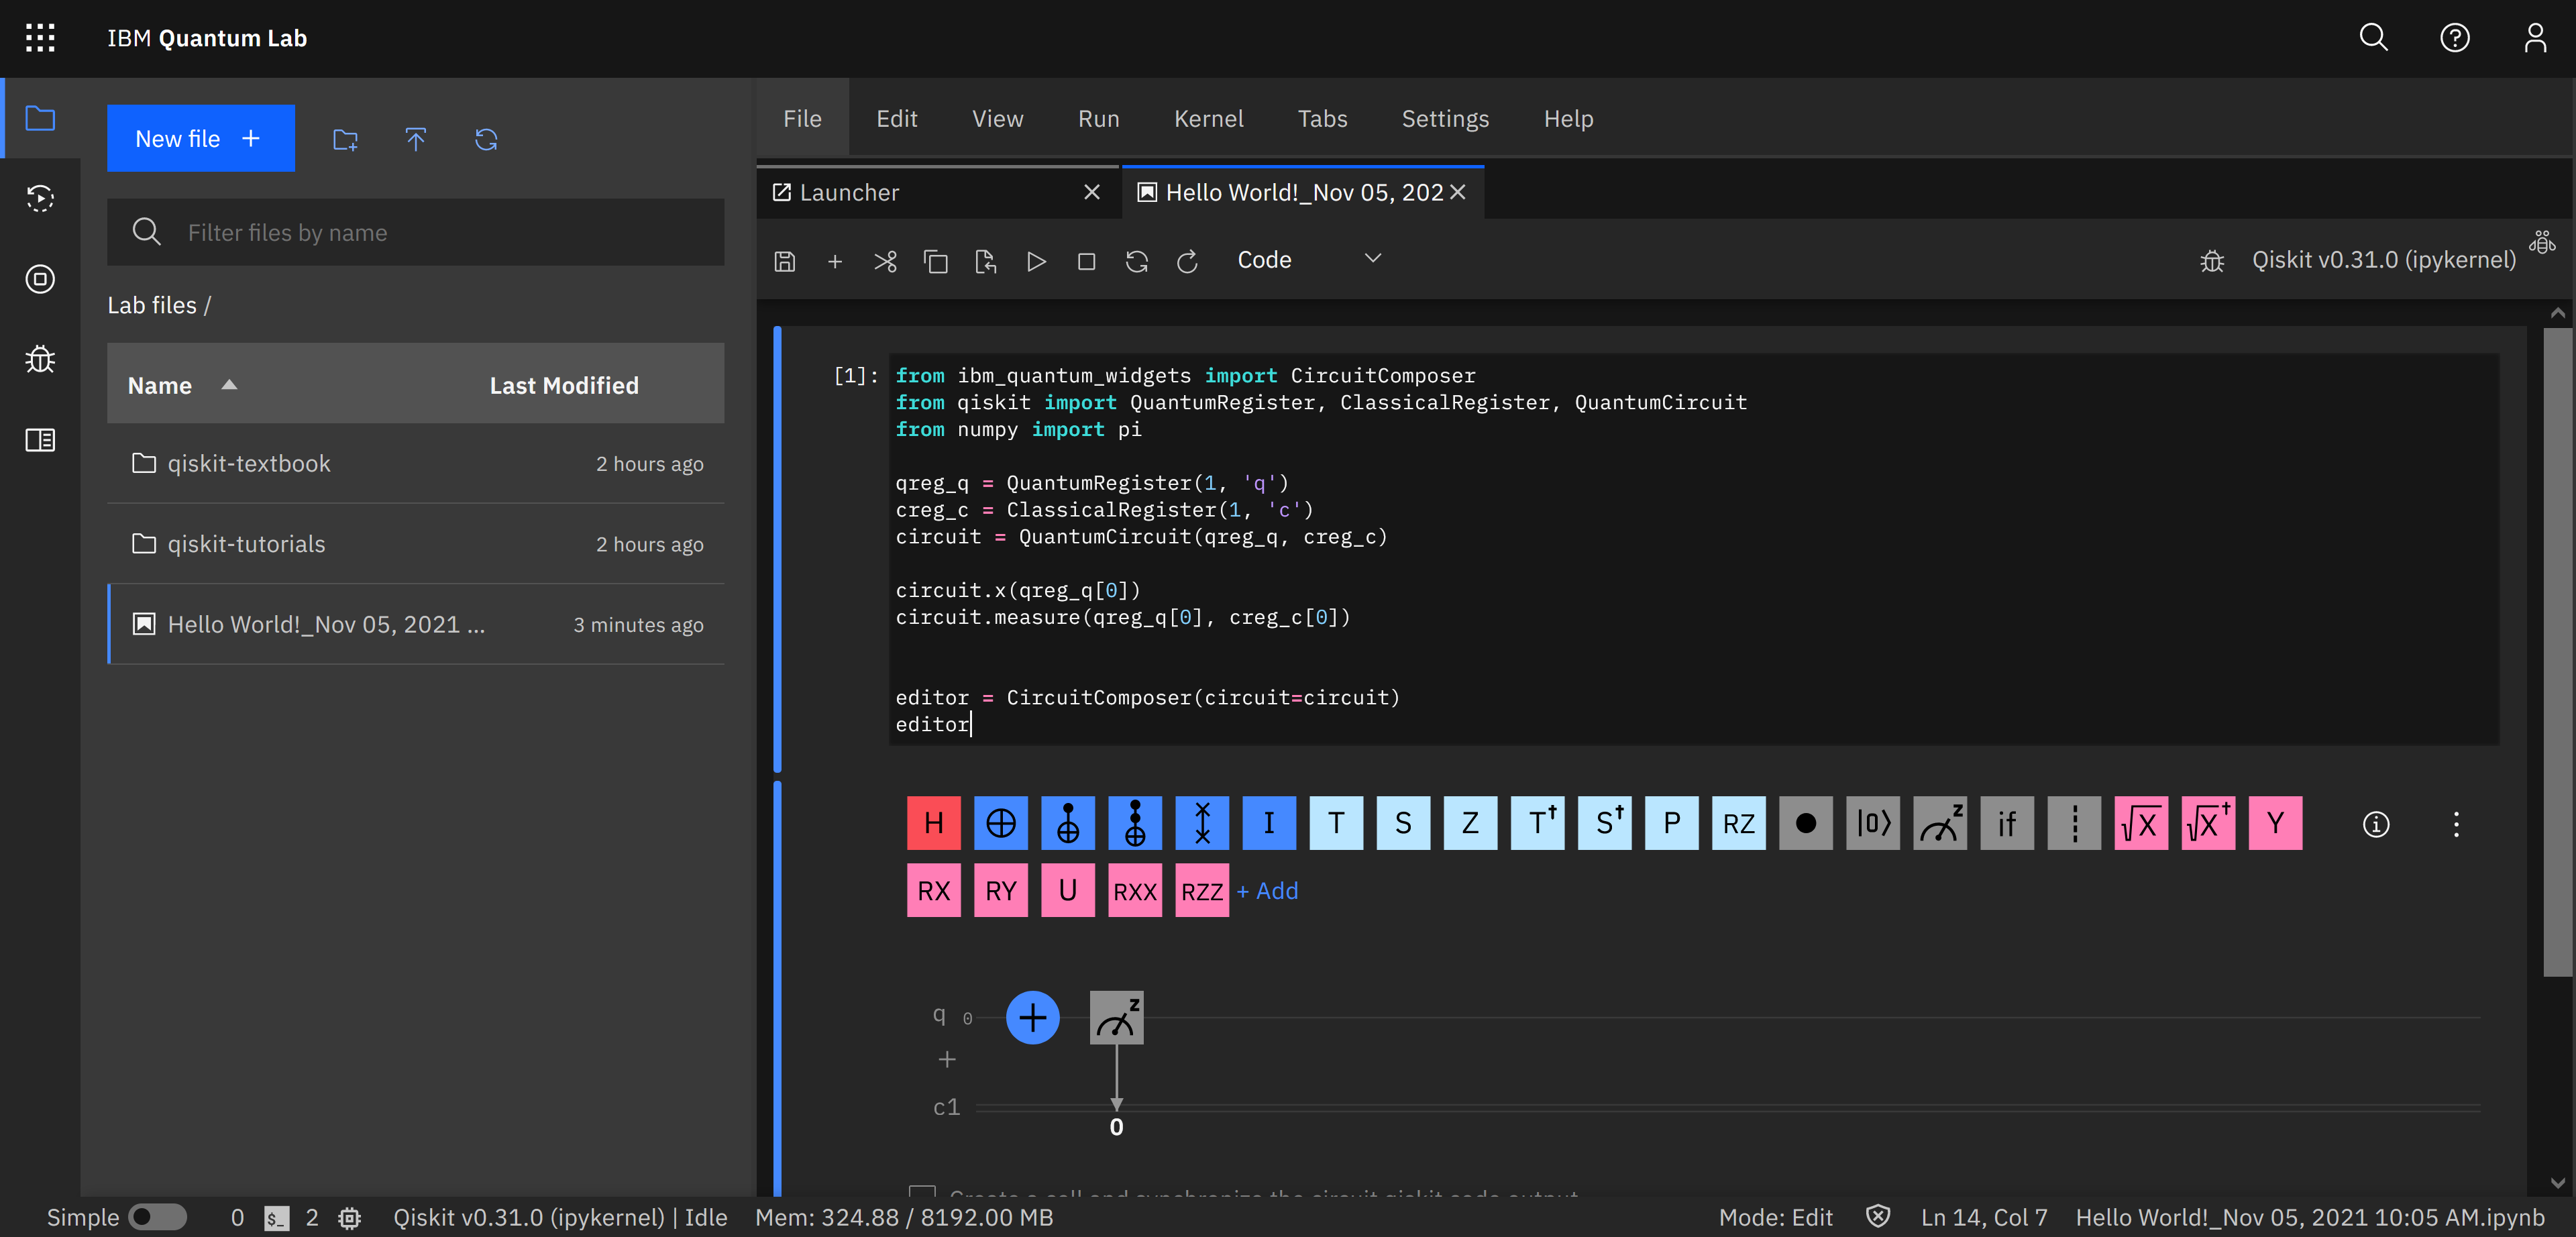
\includegraphics[width=\columnwidth]{images/HelloWorld_run_IBMQuantumLab.PNG}
\end{figure}
Now let us delete the first line and the last two lines.  Instead, let us add the line
\begin{lstlisting}[language=Python]
	circuit.draw()
\end{lstlisting}
at the end of the cell, and re-run.  You should see the previous circuit composer display changed to an image of a quantum circuit.
\begin{figure}[H]
	\includegraphics[width=\columnwidth]{images/HelloWorld-2_IBMQuantumLab.PNG}
\end{figure}

Something you may have noticed is that now, although our circuit has a measurement operation, we do not see the probabilities of all the measurement outcomes.  This is because the code so far creates a circuit, and we will need a few more lines to run this circuit.

We will run our circuits on a simulator so there is not a queue to wait in to run on physical hardware, and so we can learn what the circuits do in a noise-free environment.  Real quantum computers today are noisy, which means that they are prone to errors when performing computations.  This is why you may have heard the term \textit{Noisy Intermediate-Scale Quantum} (NISQ) to describe quantum computing today.  The expectation is that in the coming years, the noise will be low enough so that \textit{fault-tolerance} can be achieved at scale, so that quantum error correction can be performed to suppress these errors.  Therefore, the engineering challenge of scaling up quantum computers is just as much reducing noise, as increasing the number of qubits and operations between them.

To import the simulator, add `Aer' to our list of imports from Qiskit
\begin{lstlisting}[language=Python]
	from qiskit import QuantumRegister, ClassicalRegister, QuantumCircuit, Aer
\end{lstlisting}
and re-run that cell.  Then, in the cell below that, run
\begin{lstlisting}[language=Python]
	backend = Aer.get_backend('qasm_simulator')
	job = backend.run(circuit)
	result = job.result()
	print(result.get_counts())
\end{lstlisting}

You should see the output in curly brackets.  This is the \textit{counts}, a dictionary in Python which stores measurement outcomes.  By default, it runs your circuit 1024 times.  How to interpret it, is that for each binary string key in the dictionary, it gives you the number of times for which that measurement outcome was observed.
\begin{figure}[H]
	\includegraphics[width=\columnwidth]{images/HelloWorld-4_IBMQuantumLab.PNG}
\end{figure}

Just so our experiments (the name for running all these simulations) will roughly correspond to our probabilities, we can change the number of times of our circuit is run, i.e. the number of \textit{shots}, from 1024 to 100.  Keep in mind that because these are randomized, they will likely not be the exact probabilities, but they will reasonably close.  Although we could see the exact statevector, for instance if we instead used the \textit{statevector simulator}, using the QASM simulator is more realistic because on a real quantum computer, the state cannot be observed except through measurement outcomes.
\begin{lstlisting}[language=Python]
	job = backend.run(circuit, shots=100)
\end{lstlisting}

We will now see the H gate in action.  As we saw before in Figure~\ref{fig:Hgate}, it maps the $\kz0$ and $\kx{+}$ states to each other, and the $\kz1$ and $\kx{-}$ states to each other.  In other words, it maps each Z-basis state to the corresponding X-basis state, and vice versa.
You can see through matrix multiplication that
\begin{equation}
	Z = H X H
\end{equation}
and
\begin{equation}
	X = H Z H
\end{equation}

It may seem rather cumbersome to multiply matrices each time we want to figure out what a sequence of gates is doing.  Not only is it unintuitive, but we will soon see that even with small numbers of qubits, the matrices get (exponentially) large, and therefore rapidly more computationally expensive to multiply.

Thankfully, we do not have to resign ourselves to the tedium of multiplying matrices to understand what our quantum circuits are doing.  We just need to build up our toolbox so that we can use the right tool for the job.  To help us develop intuition for the Z- and X- bases, we will learn how to read, draw, and make deductions using \textbf{ZX-calculus} diagrams.  The qubit ZX-calculus is a pictorial language in which you can reason about all of qubit quantum computation.  As we continue learning, we will see how convenient of a tool these diagrams are.  As with the circuit model, we choose the convention of drawing and reading these diagrams from left to right.

We have already met the $Z$ and $X$ gates.  But have you met them in color?  The ZX-calculus was originally also called the green-red calculus, because it was invented on a whiteboard with green and red markers\footnote{In this text we will use the colors light green and darker pink, as to be easily distinguishable for the red-green colorblind.}.  Rotations about the $z$-axis Bloch sphere are colored in green, whereas rotations around the $x$-axis of the Bloch sphere are colored in red.  In the ZX-calculus, we draw Rz and Rx gates as green and red circles, respectively; they have one input wire and output wire, like how we drew them in the circuit model.  We label the circle with the \textbf{phase}, which is the angle of rotation on the Bloch sphere.

And thus, the Rz gate is drawn in the ZX-calculus as
\begin{equation*}
	\tikzfig{zxZphase}
\end{equation*}
The phase $\alpha$, in radians (i.e. any number in the range $[0,2\pi)$), is the angle of rotation about the $z$-axis on the Bloch sphere.
In matrix form, the gate in terms of $\alpha$ is:
\begin{equation}
	Z(\alpha) = \begin{bmatrix}
		1 & 0\\
		0 & e^{i\alpha}
	\end{bmatrix}
\end{equation}
This is the first example we have seen of a \textit{parametrized} gate.  This means that the gate takes in one or more parameters --- $\alpha$ in this case.

For the special case when $\alpha = 0$, no rotation occurs.  The gate is the identity gate $\mathbb{I}$ because its matrix is equal to the identity matrix.  By convention, we leave out the phase label when $\alpha = 0$:
\begin{equation}
	\tikzfig{zxZI}	
\end{equation}

There are plenty of other special cases each interesting in their own way.  One case to point out now, is that when $\alpha = \pi$, we have the $Z$ gate.  The reason why the $Z$ gate is the same gate as the $Z(\pi)$ gate, is that the $Z$ gate rotates exactly halfway ($\pi$ radians) around the $z$-axis of the Bloch sphere.  Therefore, the $Z$ gate in the ZX-calculus is drawn as
\begin{equation}
	\tikzfig{zxZ}
\end{equation}
where the right hand side of the equation is how the $Z$ gate is drawn in the circuit model.

In the opposite color, the Rx gate is drawn in the ZX-calculus as
\begin{equation*}
	\tikzfig{zxXphase}
\end{equation*}
The phase $\alpha$ is now the angle of rotation about the $x$-axis on the Bloch sphere.

We again have that $X(0) = \mathbb{I}$
\begin{equation}
	\tikzfig{zxXI}	
\end{equation}
and the $X$ gate is the same as the $X(\pi)$ gate.
\begin{equation}
	\tikzfig{zxX}
\end{equation}

% Color change rule

% We know that the $\kz0$ and $\kz1$ states are the $Z$-basis states, while the $\kx+$ and $\kx-$ states are the $X$-basis states.



%At this time, if this is your first rodeo with Qiskit, check out the `Getting started with Qiskit' Jupyter notebook to walk through how to run your circuits on hardware, before we continue.  You can navigate to it by selecting the `New file +' button which opens up the Launcher.
%\begin{figure}[H]
%	\includegraphics[width=\columnwidth]{images/Launcher_IBMQuantumLab.PNG}
%\end{figure}


\newpage
\section{When you have more than one qubit}
{\small\textit{This section will assume knowledge of vectors and matrices, and will introduce bra-ket notation alongside diagrammatic notation.  To brush up on the relevant linear algebra, visit \url{https://qiskit.org/textbook/ch-appendix/linear_algebra.html}}}

Any pure quantum state of $n$ qubits is described by a column vector of $2^n$ complex numbers --- one for each possible binary string of length $n$.  In bra-ket notation, this $n$ qubit state is denoted $\ket{v}$.
\begin{equation}
\tikzfig{ket}
\end{equation}
$v_1,...,v_{2^n}$ are complex numbers.


\bibliography{qiskit+zx.bib}
\end{document}
